\documentclass{article}

\usepackage{graphicx}
	\graphicspath{ {images/} }
\usepackage{wrapfig}
\usepackage{paralist}


\setlength{\parindent}{0pt}

\begin{document}

\begin{wrapfigure}{R}{0.40\textwidth}

\includegraphics[width=0.40\textwidth]{sarah.png}
\end{wrapfigure}
\textbf{\Large Sarah Garrell (20)} \\ \\
\textbf{Job Title: }1st year HR student\\
\textbf{Education:} High School + CEGEP\\
\textbf{Experience:}
\begin{compactitem}
\item Starbucks Barista
\item Summer camp counselor
\end{compactitem}
\textbf{Goals:}
\begin{compactitem}
\item Get her degree and work in recruiting
\item Pass accounting and finance
\end{compactitem}
\bigskip 
\textbf{Goals and Tasks user accomplishes}\\
Mostly she is worried about her finance class so anything that would help her with that would be appreciated.\\ \\
\textbf{Problem calculator solves} \\
She needs a calculator to calculate the equations for finance class. Her school does not allow her a programmable calculator so she will need to memorize the equations. She would definitely appreciate a it if she could enter the equation from left to right just like she memorized them.
\pagebreak

\begin{wrapfigure}{R}{0.4\textwidth}
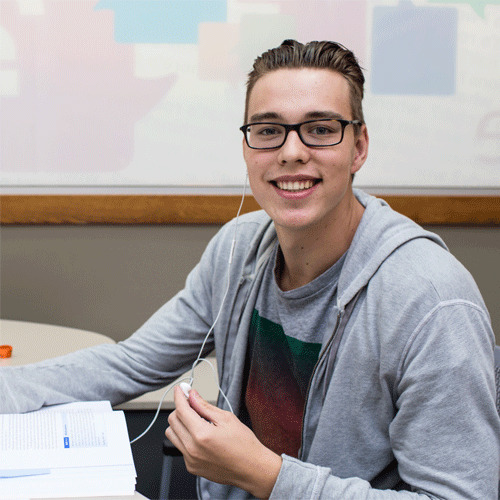
\includegraphics[width=0.4\textwidth]{kevin2.jpg}
\end{wrapfigure}
\textbf{\large Kevin Donnavan (23)} \\ \\
\textbf{Job Title: }Engineering Student\\
\textbf{Education:} 3rd Year Mechanical Engineering\\
\textbf{Experience:}
\begin{compactitem}
\item 3rd Year Mechanical Engineering
\item Summer internship as a junior structural engineer
\item Army reserves - Infantry
\end{compactitem}
\textbf{Skills:}
\begin{compactitem}
\item Problem Solving, Mathematics
\item Programming in Java, C\#, and C++
\end{compactitem}
\textbf{Goals:}
\begin{compactitem}
\item Obtain a good GPA and find a job in his field.
\end{compactitem}
\bigskip 
\textbf{Goals and Tasks user accomplishes}\\
Kevin says he just wants to get through his classes and get a decent GPA. Like everyone, his hardest classes mostly have to do with math (although he feels he is better than average). Kevin will be happy with anything that can make his math calculations easier.\\ \\
\textbf{Problem calculator solves} \\
The calculator helps Kevin get fast answers to difficult math problems he sees in class. Without a calculator, he is not sure how he would calculate the various functions that he sees on a daily basis. The calculator has to be precise enough so he can get the right answer to complex solutions of differential equations but he is not willing to wait - calculation must be near-instantaneous.
\pagebreak

\begin{wrapfigure}{R}{0.4\textwidth}
\includegraphics[width=0.4\textwidth]{tarek2.jpg}
\end{wrapfigure}
\textbf{\large Tarek Ghamzi (23)} \\ \\
\textbf{Job Title: }Engineering Student\\
\textbf{Job Title: }3rd year Electrical engineering student\\
\textbf{Education:} High School + CEGEP, currently in Electrical Engineering\\
\textbf{Experience:}
\begin{compactitem}
\item Subway
\item Pharmacist assistant
\end{compactitem}
\textbf{Skills:}
\begin{compactitem}
\item Problem Solving, Mathematics
\item Programming in C++ , and arduino 
\end{compactitem}
\textbf{Goals:}
\begin{compactitem}
\item Finish his degree with a good GPA
\item Find a job in his field
\end{compactitem}
\bigskip 
\textbf{Goals and Tasks user accomplishes}\\
Tarek claims that his main priority in life at the moment is to get his degree in Electrical Engineering. He claims that his field is heavily based on math, which he struggles with.
He aims to graduate with a higher than average GPA to gain an edge over others in his highly competitive field.\\ \\
\textbf{Problem calculator solves} \\
His calculator helps him in computing the high level mathematical functions that would take hours to solve by himself. It also helps him double check his answers for simple calculations.
Tarek claims that his calculator is with him at all times. Its accuracy, speed and comfort are of highest value to him.
\pagebreak


\begin{wrapfigure}{R}{0.40\textwidth}

\includegraphics[width=0.40\textwidth]{arash.jpg}
\end{wrapfigure}
\textbf{\Large Arash Mohajer (28)} \\ \\
\textbf{Job Title: }2nd year Avionics Engineering student \\
\textbf{Education:} High School + CEGEP, currently in University\\
\textbf{Experience:}
\begin{compactitem}
\item Completed two internships at a company that manufactures Flight Simulators
\item Worked part time as a waiter
\end{compactitem}
\textbf{Skills:}
\begin{compactitem}
\item Mathematics, Physics
\item Technical Writing
\item Some experience programming in C\# and Java
\end{compactitem}
\textbf{Goals:}
\begin{compactitem}
\item Find more internships during his degree
\item Finish his degree in a reasonable amount of time
\item Save money for his future (manage personal finance)
\end{compactitem}
\bigskip
\textbf{Goals and Tasks user accomplishes}\\
Arash wants to finish his degree in Avionics as soon as possible so that he can get a good job in a field that he enjoys. He wants to continue taking part in engineering competitions and hackathons to learn more about his field and others and to meet other like-minded individuals. He wants to manage his personal finance in order to pay off the debt that he currently has from his university tuition. \\ \\
\textbf{Problem calculator solves}
While he is more focused on graduating than getting good grades in his classes, he has many math and physics intensive classes where he relies on a calculator. He uses a calculator at school for homework, projects and exams. He also uses a calculator for conversion between different units for engineering and physics problems. At home, he uses his calculator to manage his personal finances and to plan his future spending. 
\pagebreak


\begin{wrapfigure}{R}{0.40\textwidth}

\includegraphics[width=0.40\textwidth]{victoria.jpg}
\end{wrapfigure}
\textbf{\Large Victoria Benlolo (35)} \\ \\
\textbf{Job Title: }Entrepreneur - Spa owner \\
\textbf{Education:} Business degree \\
\textbf{Experience:}
\begin{compactitem}
\item Has owned and managed a spa for 2 years
\item Worked as a financial analyst for 7 years
\end{compactitem}
\textbf{Skills:}
\begin{compactitem}
\itemsep0em 
\item Economics, Business, Finance
\item Public Speaking
\item Investing
\end{compactitem}
\textbf{Goals:}
\begin{compactitem}
\itemsep0em 
\item Maximize the profit of her business
\item Invest in new profitable endeavours 
\item She is interested in opening new spas around town once her business grows more
\item Hire new employees and continue to manage the finances of her business
\end{compactitem}
\bigskip 
\textbf{Goals and Tasks user accomplishes}\\
Victoria wants to continue to grow her business and potentially start franchising her spa to open up new locations around the city. She wants to hire new talent in order to expand her finance team. Her day-to-day includes managing employees' pay, keeping inventory of products, paying bills and managing business income. Additionally, she wants to continue investing in the stock market. \\ \\
\textbf{Problem calculator solves}
At the Spa, Victoria uses a calculator to calculate all of her business expenses, profit/loss, employee salaries, etc. A reliable calculator is very important to her. She uses a calculator to plan expenses in her future business expansion plans.  She also uses a calculator to keep track of how her personal accounts and investment portfolios are growing. 
\pagebreak

\end{document}